\section{Backgrounds}
\label{sec:od_analysis_backgrounds}
\par
Using the aforementioned energy scale, noise cut, and scaling factor, in this section the background rate in the OD is measured and attempts are made to understand what is seen.
\par
In \autoref{fig:od_random_trigger} a comparison between the observed events in the OD during the entirety of SR1 and those expected are shown from the Random Trigger.
The expected rates are those described in \autoref{sec:simulated_od_requirements} and were simulated using the ``full-propagation" chain with the result scaled by the factor determined in the previous section.
Both data and simulations were handled by the same analysis tools, with the noise cut applied to both.
Included as well in \autoref{fig:od_random_trigger} is the expected rate in the OD if the GdLS had not undergo an improve purification.
Neither case fits what is observed particularly well.
More worryingly there is a peak in the data at 100 phd which does is not in the expected rate.


\begin{figure}[]
    \centering
    \begin{tikzpicture}
    
    \begin{axis}[
        xlabel=Pulse Area,
        ylabel=Rate (Hz/5phe),
        width=15cm, height=10cm,
        xmin=0, xmax=1000,
        %ymax=1e-7, 
        ymode=log,
        legend pos=north east,
        grid=major]
            
        \addplot[only marks, mark size=0.5pt,
                 error bar legend,] 
            plot[error bars/.cd, x dir=both, x explicit]
            table[x=pulsearea,y=weight,x error=xerror, y error=yerror]
            {Data/OD_Backgrounds/background_constraints/od_data.dat};
        
        \addplot[red, const plot]
            table [x=pulsearea,y=weight]
            {Data/OD_Backgrounds/background_fit/starting_point/backgrounds_improved_purification.dat};
            
        \addplot[green, const plot]
            table [x=pulsearea,y=weight]
            {Data/OD_Backgrounds/background_fit/starting_point/backgrounds_original_purification.dat};
        
        \legend{Data, Original purification, Improved purification};
        \end{axis}
    \end{tikzpicture}
    \caption{OD pulse area spectrum from using the Random Trigger in the region. 
    Only the noise cut has been applied to the data.
    Overlaid are the expected rates from all backgrounds with the improved and original GdLS internal rates.}
    \label{fig:od_random_trigger}
\end{figure}

\par
In the remainder of this section, an attempt is made to understand what is observed and why it is different to what is expected.

\subsection{Rate Stability}

\par
To begin in the journey of understanding what is in the data, the first thing that was done was observe if the rate and distribution were stable over time.
Events from a month before the beginning of SR1 until the end were monitored every week using the Random Trigger.
The rate of events above the noise-cut, 100 keV and 200 keV were measured and are shown in \autoref{fig:OD_SR1_Rate}.
The noise-cut was applied as a base-cut, so the 100 keV is made up of the the noise-cut plus a phd cut, and similarly for 200 keV.
The three gaps in the data are when a calibrations were being performed.
This occurred three times in the region shown: just before SR1, 4 weeks into SR1, and straight after SR1.
\par
There are minor fluctuations in the noise-cut rate, but these are linked a xenon chiller and is consistent with a grounding failure, thus the behaviour is not mirrored in the 100 keV or 200 keV rates.
Importantly, over this period the OD rate remains stable, with no features in the observed distribution changing during that time.
Therefore what was shown in \autoref{fig:od_random_trigger} is the truly representative of the backgrounds in the OD.

\begin{figure}[!htbp]
    \centering
   \begin{tikzpicture}
        \begin{axis}[
        date coordinates in=x,
        %xtick=data,
        xticklabel style=
        {rotate=90,anchor=near xticklabel},
        xticklabel=\day.\month.\year,
        xlabel={Date},
        %ymin=247, ymax=250,
        y tick label style={/pgf/number format/1000 sep=},
        extra y tick style={grid=major, tick label style={xshift=-1cm}},
        ylabel={Rate (Hz)},
        date ZERO=2009-08-18,% <- improves precision!
        width=15cm,
        height=6cm,
        ]
        \addplot[smooth, error bar legend,
                 error bars/.cd,
                 y dir=both, y explicit, error bar style={color=orange}] table[x=date,y=noise, y error=noise_error] {Data/OD_Backgrounds/background_rates/random_trig_rates.txt};
                 
        \addplot[smooth, error bar legend,
                 error bars/.cd,
                 y dir=both, y explicit, error bar style={color=orange}] table[x=date,y=100kev, y error=200kev_error] {Data/OD_Backgrounds/background_rates/random_trig_rates.txt};
        
        \addplot[smooth, error bar legend,
                 error bars/.cd,
                 y dir=both, y explicit, error bar style={color=orange}] table[x=date,y=200kev, y error=200kev_error] {Data/OD_Backgrounds/background_rates/random_trig_rates.txt};
                 
        \end{axis}
    \end{tikzpicture}
    \caption{Rate in OD during and before SR1 data taking on a week-by-week basis using the Random Trigger.
    Week -1 corresponds to the month prior to SR1 when the OD PMT gains were higher.}
    \label{fig:OD_SR1_Rate_spare}
\end{figure}
%\par


\begin{figure}[!htbp]
    \centering
    \begin{tikzpicture}
        \begin{axis}[
            title=TODO: Replace with dates and errors,
            xlabel=Data taking week,
            ylabel=Rate (Hz),
            width=15cm,
            height=6cm,
            xmin=-2,
            xmax=14,
            legend style = {column sep = 10pt, legend columns = -1,}]
            \addplot[red, only marks]
                    table [x=Week,y=Rate]
                    {Data/OD_Backgrounds/background_rates/od_sr1_rate_noise.dat};
            \addlegendentry{Noise Cut};
            \addplot[blue, only marks]
                    table [x=Week,y=Rate]
                    {Data/OD_Backgrounds/background_rates/od_sr1_rate_100.dat};
            \addlegendentry{100keV};
            \addplot[green, only marks]
                    table [x=Week,y=Rate]
                    {Data/OD_Backgrounds/background_rates/od_sr1_rate_200.dat};
            \addlegendentry{200keV};
        \end{axis}
    \end{tikzpicture}
    \caption{Rate in OD during and before SR1 data taking on a week-by-week basis using the Random Trigger.
    Week -1 corresponds to the month prior to SR1 when the OD PMT gains were higher.}
    \label{fig:OD_SR1_Rate}
\end{figure}

\par
Viewing the rate in a slightly different way, the rate-per-phd for the SR1 period is shown in \autoref{fig:od_sr1_rate_vs_threshold}.
Overlaid is the expected rate of backgrounds from \autoref{tab:od_expected_rates} for 100 and 200 keV.
Interestingly the rate above 100 keV is in fairly good agreement with what was predicted in \autoref{sec:simulated_od_backgrounds}.
This is consistent with being able to set the veto energy threshold to 100 keV, assuming that achieves an appropriate veto efficiency.
However differences arise at the 200 keV level, where the expected is 62.7$\pm$5.3 Hz were as the observed is 42.5$\pm$2.1 Hz, a fairly significant difference.

\begin{figure}[]
    \centering
    \begin{tikzpicture}
        \begin{axis}[
            xlabel=OD Threshold (phd),
            ylabel=Rate (Hz),
            width=15cm, height=8cm,
            xmin=-1, xmax=55,
            ymin=0, ymax=350,
            legend pos=north east,
            grid=major]
             \addplot+[black, smooth, mark=none]
                    table [x=Threshold,y=Rate]
                    {Data/OD_Backgrounds/background_rates/od_sr1_rate_vs_threshold_smooth_line.dat};
            \addplot[black, only marks, 
                     error bar legend,
                     error bars/.cd,
                     x dir=both, x explicit, error bar style={color=black}]
                    table [x=Threshold,y=Rate, x error=XError]
                    {Data/OD_Backgrounds/background_rates/od_sr1_rate_vs_threshold_error_bars.dat};
             \addplot[dashed, mark=none, red] coordinates {(0,100) (60,100)};
             \addplot[dashed, mark=none, blue] coordinates {(17.6,0) (17.6,350)};
             \addplot[dashed, mark=none, green] coordinates {(37.5,0) (37.5,350)};
             
             \addplot[orange, only marks, 
                      error bar legend,
                      error bars/.cd,
                      y dir=both, y explicit, error bar style={color=orange}]
                      table [x=Threshold,y=Rate, y error=YError]
                      {Data/OD_Backgrounds/background_rates/od_sr1_rate_expected.dat};
             
             \legend{,SR1 Data,$<$100Hz Requirement,100 keV (17.6 phd),200 keV (37.5 phd),Expected}                
        \end{axis}
    \end{tikzpicture}
    \caption{Rate of OD backgrounds during SR1 using the Random Trigger. The noise cut has been applied. 100Hz Requirement is for a 500$\mu$s veto window as proposed in \cite{LZ_TechnicalDesignReview_ref}. Expected values are from \autoref{tab:od_expected_rates}}
    \label{fig:od_sr1_rate_vs_threshold}
\end{figure}

%%%%%%%%%%%%
\subsection{Position Reconstruction}
\par
Next we can look at the spacial distribution of events.
For any pulse it is possible to reconstruct the location of the interaction that caused the pulse by a weighted average such as:
\begin{equation}
    x = \frac{\sum{\text{Ch}_{\text{phd}} * \text{Ch}_\text{x}}}{\sum{\text{Ch}_\text{phd}}} 
\label{eq:OD_xy_position}
\end{equation}
where Ch$_{phd}$ is the phd of a PMT channel and Ch$_{x}$ is the position of the PMT.
Due to scheduling constraints associated with SR1, there was an insufficient variety of calibration sources were used at varying \{$x,y,z$\} positions in order to adequately determine the resolution of this approach, but it is something a future calibration campaign may be able to tackle. 
Additionally, this approach does not take into account the OCV in the centre of the detector, so reconstructed pulses will have an incorrect position, but the correct shape.
The OCV can be taken into account by converting coordinate system, but has explicitly not been done here due to the lack of knowledge in the actual resolution of this approach.
Regardless however, this approach does provide an insight in a way not thought possible based upon optical simulations.

\par
This approach was performed on slices in phd-space, the result of which can be seen in \autoref{fig:od_backgrounds_position_reconstruction}.
The first region focuses on the peak at 100 phd ($\backsim$ 0.5 MeV).
The second region focuses on the area above 2 MeV, where cavern-$\gamma$s should dominate.

\begin{figure}[!htbp]%
\centering
\begin{tikzpicture}
\centering
  \begin{groupplot}[%view={0}{90},
    group style = {group size = 2 by 3,vertical sep=3cm,
                   horizontal sep=1.5cm},
                   height=6cm, width=0.5\textwidth]
    \nextgroupplot[
            ylabel=Rate (Hz),
            xlabel=Pulse Area (phd),
            width=0.95\textwidth,
            height=6cm,
            %xshift=0.5\textwidth,
            xmin=0, xmax=800,
            ymin=1e-4, ymax=1e3,
            ymode=log,
            ]
            \addplot[only marks, mark size=1.0pt] 
            plot[error bars/.cd, x dir=both, x explicit]
            table[x=pulsearea,y=weight,x error=xerror, y error=yerror]
            {Data/OD_Backgrounds/background_constraints/od_data.dat};
            
            \addplot[dashed, mark=none, name path=A,blue] coordinates {(75,0.00001) (75,10000)};
            \addplot[dashed, mark=none, name path=B,blue] coordinates {(125,0.00001) (125,10000)};
            \addplot[dashed, mark=none, name path=C,green] coordinates {(500,0.00001) (500,10000)};
            \addplot[dashed, mark=none, name path=D,green] coordinates {(1000,0.00001) (1000,10000)};

            \addplot[blue!50] fill between[of=A and B];
            \addplot[green!50] fill between[of=C and D];
            
    \nextgroupplot[group/empty plot]

    \nextgroupplot[colorbar, 
    colorbar style={title=Rate (Hz),ymode=log,},
    width=0.4\textwidth, view={0}{90},
    xshift=-0.3\textwidth,
    ylabel=Z (cm),
	xlabel=R (cm),
	y label style={at={(axis description cs:-0.13,0.5)},anchor=near ticklabel},]
    \addplot3[
		surf,
		shader=flat corner,
		mesh/cols=50,
		mesh/ordering=rowwise,
		point meta = {z>1 ? nan : z}
		] file {Data/playground/alpha_peak_r_z.csv};
	\node [rotate=90] at (axis cs:0,1050) {Region 1};
	\nextgroupplot[colorbar, 
	colorbar style={title=Rate (Hz),ymode=log,},
	width=0.4\textwidth, view={0}{90},
    xshift=-0.5\textwidth, %yshift=1.5cm,
    ylabel=Y (cm),
	xlabel=X (cm),
	y label style={at={(axis description cs:-0.13,0.5)},anchor=near ticklabel},]
    \addplot3[
		surf,
		shader=flat corner,
		mesh/cols=54,
		mesh/ordering=rowwise,
		point meta = {z>1 ? nan : z}
		] file {Data/playground/alpha_peak_x_y.csv};

    \nextgroupplot[colorbar, 
    colorbar style={title=Rate (Hz),ymode=log,},
    width=0.4\textwidth, view={0}{90},
    ylabel=Z (cm),
	xlabel=R (cm),
	y label style={at={(axis description cs:-0.13,0.5)},anchor=near ticklabel},]
    \addplot3[
		surf,
		shader=flat corner,
		mesh/cols=50,
		mesh/ordering=rowwise,
		point meta = {z>1 ? nan : z}
		] file {Data/playground/rg_th232_r_z.csv};
		
	\nextgroupplot[colorbar, 
	colorbar style={title=Rate (Hz),ymode=log,},
	width=0.4\textwidth, view={0}{90},
	ylabel=Y (cm),
	xlabel=X (cm),
    y label style={at={(axis description cs:-0.13,0.5)},anchor=near ticklabel},]
    \addplot3[
		surf,
		shader=flat corner,
		mesh/cols=54,
		mesh/ordering=rowwise,
		point meta = {z>1 ? nan : z}
		] file {Data/playground/rg_th232_x_y.csv};
   
  \end{groupplot}
  
  \node at ($(group c1r2) + (-1.0cm, 3.5cm)$) {\textbf{Region 1 (blue)}};
  \node at ($(group c1r3) + (-1.0cm, 3.5cm)$) {\textbf{Region 2 (green)}};
  
\end{tikzpicture}
\caption{Position Reconstruction of pulses from various regions in pulse area space defined in the top plot. 
         Each pulse has had the noise cut applied and the position reconstructed using \autoref{eq:OD_xy_position}.}
\label{fig:od_backgrounds_position_reconstruction}
\end{figure}

\par
There are two useful observations in both regions.
Firstly, in $r-z$ there is a clear bias to events at the bottom of the detector.
This is consistent with cavern-$\gamma$s distribution shown in \autoref{fig:cavern_gamma_position_distribution}.
This indication that the cavern-$\gamma$s is the most significant contributor, again in agreement in the prediction (\autoref{tab:od_expected_rates}).
Secondly, in $x-y$ there is an elevated rate of events in \{$+x,+y$\}.
This can be understood easiest by labelling the SATs with letters A-D starting from \{$+x,+y$\} and going around clockwise.
Using this labelling, over the period of SR1, SAT A has a rate in excess of 8\% higher than any of the other tanks, with SAT B seeing the next highest rate (3\% higher than the mean).
Both SATs C and D saw an equivalent rate.
In \autoref{fig:OD_conduit_geometry}, the SAT placement are shown along with the conduits.
SAT A and SAT B are the only tanks which are obstructed by a single conduit, additionally both tanks cover an entire BAT and TAT.
The CSD-ports and the OCV legs block the other SATs from the TATs and BATs.
This results in the light having a more direct path to more PMTs and therefore higher probability of detection.

\begin{figure}[!htbp]
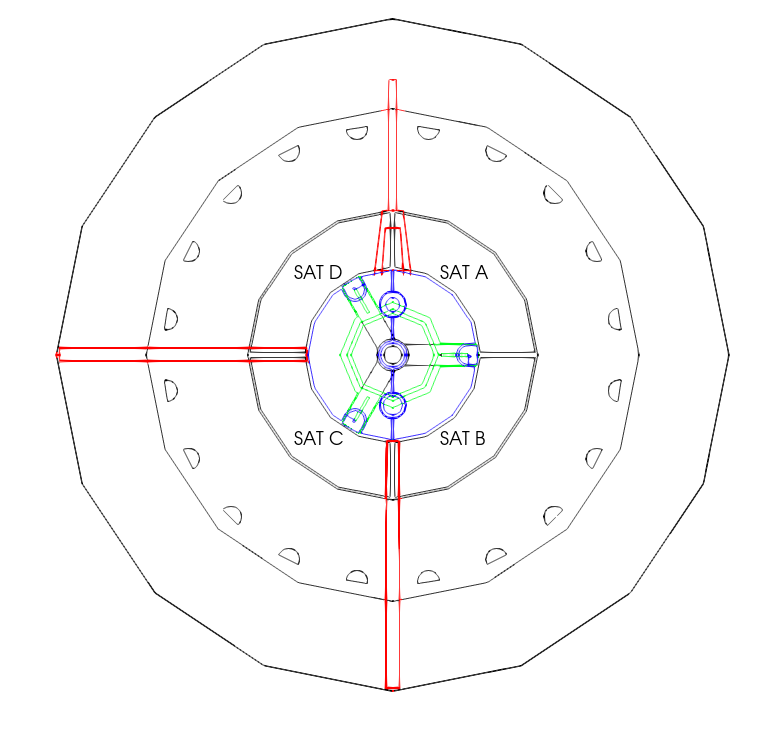
\includegraphics[width=\textwidth]{Figures/Geometry/geometry_with_conduits.png}
\centering
\caption{LZ geometry schematic. The OD geometry excluding the BATs and TATs is shown in black. The BATs and bottom on OCV are shown in green. The TATs, CSD ports and PMT conduits in blue. The DD calibration conduits and the High-Voltage feed through for the TPC are shown in red.}
\label{fig:OD_conduit_geometry}
\end{figure}


\par
As a way of suppressing cavern-$\gamma$'s is to take a slice in $z$, taking events reconstructed to be in the middle of the side tanks.
The resultant pulse area spectrum is shown in \autoref{fig:od_data_pulsearea_middle_tank}.
When compared to \autoref{fig:od_backgrounds_position_reconstruction} additional features appear around 300 phd.
These are consistent with ${}^{60}Co$ which is present in the OCV.
In future it may be possible to accurately measure the rate of this using this volume cut, but that will require a more dedicated calibration campaign, as the true quantity of the SAT selected is not clear.

\begin{figure}[!htbp]
    \centering
    \begin{tikzpicture}
    
    \begin{axis}[
        xlabel=Pulse Area,
        ylabel=Rate (Hz/5phe),
        width=15cm, height=10cm,
        xmin=0, xmax=800,
        ymin=1e-4, ymode=log,
        legend pos=north east,
        grid=major]
            
        \addplot[only marks, mark size=0.5pt] 
            plot[error bars/.cd, x dir=both, x explicit]
            table[x=pulsearea,y=rate,x error=x_error, y error=y_error]
            {Data/OD_Backgrounds/background_constraints/od_data_pulsearea_middle_tank_binwidth_5.dat};
            
        \end{axis}
    \end{tikzpicture}
    \caption{OD pulse area spectrum from pulses reconstructed to the middle of the OD side tanks, suppressing the rate from Cavern-$\gamma$'s.}
    \label{fig:od_data_pulsearea_middle_tank}
\end{figure}

\par
We now focus our attention more directly at specific backgrounds that are expected, to try and constraint them.

\subsection{$\gamma$ constraints}
\par
Another area to look at is high energy $\gamma$'s, from ($\alpha$,$\gamma$) reactions, which were discussed in \autoref{sec:cavern_gamma_generator}.
In \autoref{fig:od_high_energy} a the expected and observed rate per pulse area above 400 phd is shown.
The rate of events expected is significantly greater than that observed.
The findings here support the discussion in \autoref{sec:cavern_gamma_generator}, that the statistical model used does not extend well to ${}^{17}$O.
However, there are still features seen in data between 1000 and 1800 phd that are not accounted for in simulations.
These features have attributed to neutron captures on the Fe of the water tank (which is made of steel) producing high energy $\gamma$'s \autoref{iron_neutrons_ref}.
These neutrons originate primarily from the ${}^{252}$Cf calibration source, which was stored in a movable safe underground during SR1.
It was moved location within the cavern during SR1 which matches with a change in the reconstructed position of these events.
Backgrounds of this type were not previously considered within LZ, though are of great importance in fusion experiments \cite{iter_neutrons_ref}.
Primarily due to the source safe placement during SR1, it was not possible to determine if there was any fluctuation in the high-energy $\gamma$-rate during SR1.

\begin{figure}[]
    \centering
    \begin{tikzpicture}
    
    \begin{axis}[
        xlabel=Pulse Area (phd),
        ylabel=Rate (Hz),
        width=15cm, height=10cm,
        xmin=400, xmax=3000,
        %ymax=1e-7, 
        ymode=log,
        legend pos=north east,
        grid=major]
            
        \addplot[only marks, mark size=0.5pt,
                 error bar legend,] 
            plot[error bars/.cd, x dir=both, x explicit]
            table[x=pulsearea,y=weight,x error=xerror, y error=yerror]
            {Data/OD_Backgrounds/background_constraints/od_data.dat};
            
        \addplot[red, const plot]
            table [x=pulsearea,y=weight]
            {Data/OD_Backgrounds/background_fit/starting_point/backgrounds_original_purification.dat};
            
        \legend{Data, Expectation};
        \end{axis}
    \end{tikzpicture}
    \caption{OD pulse area spectrum for high energy $\gamma$ events compared to the expected rate.
             The events observed in data between 1000 and 1800 phd are high energy $\gamma$-rays from neutron capture the iron.}
    \label{fig:od_high_energy}
\end{figure}


%%%%%%%%%%%%
\subsection{$\alpha$ constraints}
\par
Although the exact rate of GdLS is not known, it is possible to constrain some.
Notably, decays within the U and Th decay chains all have an isotope in them with a half-life shorter than the LZ event window.
As such it is possible to observe two decays in the same event from the same decay chain.
There are 3 possible decays, summarised in \autoref{tab:od_constrainable_decays_in_data}.
However, in reality only ${}^{214}$Bi$ \to {}^{214}$Po and ${}^{219}$Rn $\to {}^{215}$Po can be searched for as the interactions from ${}^{212}$Bi $\to {}^{212}$Po are close enough together that they will be merged into one pulse.

\begin{table}[!htbp]
    \centering
    \begin{tabular}{c|c|c|c|c|c}
        \multirow{2}{*}{Decay Pair (chain)}                    & \multicolumn{2}{c|}{First Decay}   & \multicolumn{3}{c}{Second Decay}    \\ 
                                                               & Decay    & Energy (MeV) & Decay    & Energy (MeV) & half-life ($\mu$s) \\ \hline
        ${}^{214}Bi \to {}^{214}Po$ (${}^{238}U_{m}$)          & $\beta$  & 3.27         & $\alpha$ & 7.83         & 160   \\ 
        ${}^{219}Rn \to {}^{215}Po$ (${}^{235}U_{l}$)          & $\alpha$ & 6.95         & $\alpha$ & 7.53         & 1800  \\ 
        ${}^{212}Bi \to {}^{212}Po$ (${}^{232}Th_{l}$)         & $\beta$  & 2.25         & $\alpha$ & 8.95         & 0.3
    \end{tabular}
    \caption{Th and U decay chain pairs with half-lives within the LZ event window of 4.5ms. See \autoref{fig:decay_chains} for the complete Decay Chains.}
    \label{tab:od_constrainable_decays_in_data}
\end{table}

\par
The decay pairs can be searched for by looking for pulses which are reconstructed to be close to each other in position.
The position requirement is to reduce the impact of coincident interactions and decays in other areas of the OD.
As the second decay is an $\alpha$ it does not have significant penetrating power so the interaction will be close to where the initial decay was.
The cut implemented loosely to account for potential variable inefficiencies in the position reconstruction with $z$ and $\theta$.
The final selection used was a $z_{\text{diff}} < 100$ and $\theta_{\text{diff}} < 1.0$, where diff refers to the difference between pulses.
The result of this is shown in \autoref{fig:od_bipo_alphas_2d}.
Only pulses above 200keV in visible energy are included.

\begin{figure}[!htbp]%
\centering
\begin{tikzpicture}
\centering
  \begin{axis}[
    height=10cm, width=10cm,
    view={0}{90},
    ylabel={Second Pulse (phd)},
    xlabel={First Pulse (phd)},
    colorbar,
    colorbar style={ylabel={Rate (Hz)},ymode=log,},
    ]
    \addplot3[
      surf,
      shader=flat corner,
	  mesh/cols=40,
	  mesh/ordering=rowwise,
	  point meta = {z<0.0000001 ? nan : z}
    ] file {Data/OD_Backgrounds/background_constraints/rnpo_rate_2d.dat};

  \end{axis}
\end{tikzpicture}
\caption{Relationship of pulses reconstructed in close proximity to each other. Only pulses above 200 keV have been included.}
\label{fig:od_all_pulse_pairs_2d}
\end{figure}

\begin{figure}[!htbp]%
\centering
\begin{tikzpicture}
\centering
  \begin{groupplot}[%view={0}{90},
    group style = {group size = 1 by 2,vertical sep=1.5cm,
                   horizontal sep=1.5cm},
                   height=6cm, width=0.5\textwidth]

	\nextgroupplot[height=10cm, width=10cm,
    view={0}{90},
    ylabel={Second Pulse (phd)},
    xlabel={First Pulse (phd)},
    colorbar,
    colorbar style={ylabel={Rate (Hz)},ymode=log,},
    ]
    \addplot3[
      surf,
      shader=flat corner,
	  mesh/cols=40,
	  mesh/ordering=rowwise,
	  point meta = {z<0.0000001 ? nan : z}
    ] file {Data/OD_Backgrounds/background_constraints/rnpo_rate_2d.dat};
    
    
    \nextgroupplot[height=10cm, width=10cm,
    view={0}{90},
    ylabel={Second Pulse (phd)},
    xlabel={First Pulse (phd)},
    colorbar,
    colorbar style={ylabel={Rate (Hz)},ymode=log,},
    ]
    \addplot3[
      surf,
      shader=flat corner,
	  mesh/cols=40,
	  mesh/ordering=rowwise,
	  point meta = {z<0.0000001 ? nan : z}
    ] file {Data/OD_Backgrounds/background_constraints/bipo_rate_2d.dat};
   
  \end{groupplot}
\end{tikzpicture}
\caption{Relationship of pulses reconstructed in close proximity to each other. Only pulses above 200 keV have been included.
         \textbf{Top:} All pulses-pairs within 800 $\mu$s of each other. The distribution is from ${}^{214}$Bi $\to {}^{214}$Po.
         \textbf{Bottom:} All pulse-pairs with more than 800 $\mu$s time separation between them. The distribution left is from ${}^{219}$Rn $\to {}^{215}$Po.
         }
\label{fig:od_time_dependent_pulses_2d}
\end{figure}



\par
The distribution around 170 phd in both pulses correspond to the $\alpha$'s in the ${}^{235}U_{l}$ chain.
Although less clear, the second pulse contains a second $\alpha$ around the same place, and a $\beta$ spectrum in the first pulse.
This becomes easier to see in when the features are extracted as is shown in \autoref{od_bipo_alphas}.

\begin{figure}[!htbp]%
\centering
\begin{tikzpicture}
\centering
    \begin{axis}[
            ylabel=Rate (Hz/2keV),
            xlabel=Energy (MeV),
            width=15cm,
            height=8cm,
            grid=major,
            xmin=0, xmax=3,
            ymin=1e-4, ymode=log,]
            
        \addplot[red, only marks, mark size=1, 
                 error bars/.cd,
                 y dir=both, y explicit, error bar style={color=black}]
            table [x=energy,y=rate,y error plus index=2, y error minus index=3]
            {Data/OD_Backgrounds/background_constraints/od_bipo_first_alpha.dat};
            
        \addplot[blue, only marks, mark size=1, 
                 error bars/.cd,
                 y dir=both, y explicit, error bar style={color=black}]
            table [x=energy,y=rate,y error plus index=2, y error minus index=3]
            {Data/OD_Backgrounds/background_constraints/od_bipo_second_alpha.dat};
                
    \end{axis}
            
\end{tikzpicture}
    \caption{$\alpha$ energies in from BiPo and RnPo.}
    \label{fig:od_bipo_alphas}
\end{figure}

\par
The second pulse distribution peak is broadened due to two Gaussian's contributing to it, from two $\alpha$'s.
One from ${}^{214}Po$ and one from ${}^{215}Po$.
We are able to constrain the rate of these events by using a reverse search, finding the second $\alpha$ in the energy range and then looking for the first decay.
This gives a rate of 98$\pm$2.5 $\mu$Hz for ${}^{214}Bi \to {}^{214}Po$, which is within 50\% that expected from the 'improved purification' (see \autoref{sec:simulated_od_requirements}).
Measuring the rate of ${}^{219}Rn \to {}^{215}Po$ is performed in a similar way giving a rate of 7.7$\pm$1.2 $\mu$Hz, though with an addition time constraint accounting for several decay-constants worth of time which is lower than the decay half-life of ${}^{214}Po$.
The selection of this data is shown in \autoref{fig:od_bipo_alphas_2d}.
This is again within 50\% of that from the 'improved purification', and so the assumption can be made that this purification was done, and that the estimated rates can be assumed true for all decays.


\par
Importantly, these constraints indicate that the $\alpha$-peak seen in \autoref{fig:od_random_trigger} is not from those subchains, as the rate would be too low.
This opens up the possibility that it is from ${}^{210}$Po from the late chain of ${}^{238}$U. 
This claim appears at odds with the relatively low internal rate of ${}^{238}$U.
However, it is known and measured that there is significant Rn in the cavern air, and as previously discussed (\autoref{sec:od_construction_sec}) the acrylic tanks were open to the air for long periods prior to installation.
There was opportunity for decay daughters to plate-out on the inside of the acrylic tanks, a feature that is of great concern within the TPC \cite{radon_plateout_ref}.
${}^{210}$Pb is the only long-lived particle in the Radon chain, with a half-life in excess of 22-years. 
The remainder of the isotopes would drastically reduce in abundance after a few weeks, leaving only ${}^{210}$Pb daughters visible, at a sustained rate.
This allows the acrylic holding the scintillator to act as a reservoir, providing a constant supply of $\alpha$ decays from ${}^{210}$Po.
LZ is not alone in having experienced this, with KamLAND measuring a higher than expected rate of ${}^{238}$U$_l$ decays \cite{KamLAND_LS_contaminants_ref}.

\par
Although it is unexpected to see a four $\alpha$'s, it becomes possible to perform an $\alpha$ energy calibration, and will be continuously measurable during all Science runs, without the need for Science data taking to be stopped.
An additional advantage is that PMT gain-drift will be more easily detectable.
The observed energy of each of the $\alpha$'s verse the observed energy are shown in \autoref{fig:od_alpha_quenching}, the Birk's law fit is also provided using the parameters in \autoref{tab:Birks_law_parameters}.
It can be seen that the parameters taken from pure LAB remain in good agreement with Gd-doped LAB used here.
This also isolates the difference between observed data and simulations to light propagation.

\begin{figure}[!htbp]%
\centering
\begin{tikzpicture}
\centering
    \begin{axis}[
            ylabel=Visible Energy (MeV),
            xlabel=Particle Energy (MeV),
            width=15cm,
            height=8cm,
            grid=major,
            xmin=0, xmax=10,
            ymin=0,
            legend pos=north west,
            ]
            
        % Birks Fit
        \addplot[red]
            table [x=Energy,y=Quenched]
            {Data/GdLS_Physics/Quenching/alpha.dat};
        \addplot[black, only marks, mark size=1, 
                 error bars/.cd, error bar style={color=black},
                 y dir=both, y explicit,]
            table [x=energy,y=observed,y error plus index=2, y error minus index=3]
            {Data/OD_Backgrounds/background_constraints/od_alpha_energies.dat};
        \legend{Birk's, Measured};
    \end{axis}
            
\end{tikzpicture}
    \caption{Observed energy vs particle energy from $\alpha$ particles.
             The expected quenching from Birk's Law using the parameters in \autoref{tab:Birks_law_parameters} is shown to be in good agreement with what is observed.}
    \label{fig:od_alpha_quenching}
\end{figure}

\subsection{${}^{152}Gd$}
\par
The final background that can be constrained is ${}^{152}Gd$, which produces a 2.2 MeV $\alpha$ decay ($\approx$ 120 keV visible energy).
The GdLS is loaded with 0.1\% (by mass) of natural Gadolinium.
With a total mass of GdLS used in the detector this corresponds to 16000kg, and ${}^{152}Gd$ has a natural abundance of 0.2\%, this gives a maximum possible rate of 27Hz, where there is a 5\% uncertainty on the doping by mass.
\par
Unfortunately this does not constrain this region.
Of particular note are ${}^{14}C$, a $\beta$ decay with an end-point of 156 keV, and ${}^{147}Sm$ which decays via the emission of a 2.3 MeV $\alpha$.
All three were previously measured in the LS screener campaign, with ${}^{14}$C being the dominant contributor (>100 Hz).

\subsection{Background Fitting}
\par
Given the constraints placed on rates, it is possible to fit the expected distribution to data. 
The fit was limited to only include the region of the simulation which is approximately correct with the data. 
As such, the high energy, above 600phd ($\gtrsim$ 2.5MeV) was excluded, and a low energy cut was 20phd was used.
\par
In order to keep the number of fit parameters down, all detector components were in combined. 

Given the mitigation procedure described in \autoref{sec:od_construction_sec}, the contamination is likely to be minimal from these components.
\par
Another source, ${}^{7}Be$, which has been considered in fits from similar experiments has been excluded here.
As it only has a half-life of 50-days, and the OD was not in a stable running condition until nearly a year after filling, it has been assumed that the contribution from ${}^{7}Be$ would be negligible \cite{be7_decay_ref}.
\par
The cavern-$\gamma$'s were allowed to float within the uncertainties they were measured in \cite{LZ_Gamma_Ray_Background_ref}.
The ${}^{235}U_e$, ${}^{235}U_l$, ${}^{238}U_e$, ${}^{238}U_m$, ${}^{238}U_l$, ${}^{232}Th_e$, ${}^{232}Th_l$ where constrained to be in equilibrium with the sub-chains, and constrained by the LS Screener result or the measured $\alpha$-rate here, with the exception of ${}^{238}U_l$ which was able to float freely.
The internal decays were left to float as freely as possible.

\begin{figure}[!htbp]%
\centering
\begin{tikzpicture}
\centering
    \begin{groupplot}[
    group style = {group size = 1 by 2,vertical sep=1.0cm}
    ]
    \nextgroupplot[
            ylabel=Rate (Hz/5phd),
            xlabel=,
            xmajorticks=false,
            width=15cm,
            height=10cm,
            grid=major,
            xmin=0, xmax=700,
            ymin=1e-2, ymax=100,
            ymode=log,
            legend style = { column sep = 10pt, legend columns = 3, cells={line width=1.5pt}}
            ]
        \addplot[only marks, mark size=1.0pt, black, error bar legend] 
            plot[error bars/.cd, x dir=both, x explicit, ]%y dir=both, y explicit, ]
            table[x=pulsearea,y=weight,x error=xerror, y error=yerror]
            {Data/OD_Backgrounds/background_constraints/od_data.dat};
        \addlegendentry{data};
            
        \addplot[const plot, teal]
            table [x=bin_low, y=weight]
            {Data/OD_Backgrounds/background_fit/fit_components/rg_k40.dat};
        \addlegendentry{Cavern ${}^{40}$K};
        \addplot[const plot, cyan]
            table [x=bin_low, y=weight]
            {Data/OD_Backgrounds/background_fit/fit_components/rg_u238.dat};
        \addlegendentry{Cavern ${}^{238}$U};
        \addplot[const plot, green]
            table [x=bin_low, y=weight]
            {Data/OD_Backgrounds/background_fit/fit_components/rg_th232.dat};
        \addlegendentry{Cavern ${}^{232}$Th};
        \addplot[const plot, lime]
            table [x=bin_low, y=weight]
            {Data/OD_Backgrounds/background_fit/fit_components/ocv.dat};
        \addlegendentry{Detector};
        \addplot[const plot, yellow]
            table [x=bin_low, y=weight]
            {Data/OD_Backgrounds/background_fit/fit_components/Internal_improved_u238_early.dat};
        \addlegendentry{${}^{238}$U early};
        \addplot[const plot, pink]
            table [x=bin_low, y=weight]
            {Data/OD_Backgrounds/background_fit/fit_components/Internal_improved_u238_late.dat};
        \addlegendentry{${}^{238}$U late};    
        \addplot[const plot, olive]
            table [x=bin_low, y=weight]
            {Data/OD_Backgrounds/background_fit/fit_components/Internal_improved_th232_early.dat};
        \addlegendentry{${}^{232}$Th early};
        \addplot[const plot, brown]
            table [x=bin_low, y=weight]
            {Data/OD_Backgrounds/background_fit/fit_components/Internal_improved_C14.dat};
        \addlegendentry{${}^{14}$C};
        \addplot[const plot, orange]
            table [x=bin_low, y=weight]
            {Data/OD_Backgrounds/background_fit/fit_components/Internal_improved_Gd152.dat};
        \addlegendentry{${}^{152}$Gd + ${}^{147}$Sm};
        \addplot[const plot, violet]
            table [x=bin_low, y=weight]
            {Data/OD_Backgrounds/background_fit/fit_components/total_fit.dat};
        \addlegendentry{fit};
            
            
    \nextgroupplot[
            ylabel=Ratio (data/fit),
            xlabel=Pulse Area (phd),
            width=15cm,
            height=5cm,
            grid=major,
            xmin=0, xmax=700,
            ymin=0, ymax=2,
            ]
        \addplot[only marks, mark size=1.0pt, black, error bar legend] 
            plot[error bars/.cd, y dir=both, y explicit]
            table[x=bin,y=value, y error=error]
            {Data/OD_Backgrounds/background_fit/fit_components/ratio.dat};
        
        \addplot[black, mark=none, dashed] coordinates {(20,-1) (20,3)};
        \addplot[black, mark=none, dashed] coordinates {(600,-1) (600,3)};
        
    \end{groupplot}
\end{tikzpicture}
    \caption{Result of fit to data.
             \textbf{Top:} Contribution from each source. Only components with a contribution greater than 1 Hz have been included.
             \textbf{Bottom:} Ratio of fit to data. The dashed lines indicate the fit region.
             In generally there is good agreement.}
    \label{fig:od_background_fit_to_data}
\end{figure}


\begin{table}[!htbp]
    \centering
    \begin{tabular}{c|c|c|c}
        Source               &  Decay Type(s)             & Expected Rate (Hz)       & Fitted Rate (Hz) \\ \hline
        \multicolumn{4}{l}{\textbf{Externals}} \\
        Cavern ${}^{238}$U   & $\gamma$                   & 13.98                      & 22.54                    \\ 
        Cavern ${}^{232}$Th  & $\gamma$                   & 20.06                      & 11.74                    \\ 
        Cavern ${}^{40}$K    & $\gamma$                   & 6.70                       & 13.33                    \\ 
        Detector             & $\gamma$,$\beta$           & 2.29                       & 4.59                    \\
        \multicolumn{4}{l}{\textbf{Internals}} \\
        ${}^{238}U_{e}$     & $\gamma$,$\alpha$,$\beta$  & 0.71                      & 2.57                    \\ 
        ${}^{238}U_{m}$     & $\gamma$,$\alpha$,$\beta$  & 0.30                      & 0.03                    \\
        ${}^{238}U_{l}$     & $\gamma$,$\alpha$,$\beta$  & 0.11                      & 7.60                 \\
        ${}^{235}U_{e}$     & $\gamma$,$\alpha$,$\beta$  & 0.82                      & 0.08                    \\
        ${}^{235}U_{l}$     & $\gamma$,$\alpha$,$\beta$  & 0.52                      & 0.12                    \\
        ${}^{232}Th_{e}$    & $\gamma$,$\alpha$,$\beta$  & 0.12                      & 1.2                    \\
        ${}^{232}Th_{l}$    & $\gamma$,$\alpha$,$\beta$  & 0.15                      & 0.02                    \\
        ${}^{40}K$          & $\gamma$,$\beta$           & 0.05                      & 0.05                    \\
        ${}^{14}C$          & $\beta$                    & 108.25                    & 98.32                     \\
        ${}^{176}Lu$        & $\gamma$,$\beta$           & 0.17                      & 1.65                    \\
        ${}^{147}Sm$        & $\alpha$                   & 14.6                      & 13.15                    \\
        ${}^{152}Gd$        & $\alpha$                   & 27.2                      & 18.54                     
        
    \end{tabular}
    \caption{Th and U decay chain pairs with half-lives within the LZ event window of 4.5ms. See \autoref{fig:decay_chains} for the complete Decay Chains.}
    \label{tab:od_constrainable_decays_in_data}
\end{table}